\documentclass[11pt,a4paper]{article}
\usepackage[margin=1in]{geometry}
\usepackage{beamerarticle}
\usepackage{kotex}
\usepackage{amsmath,amssymb}
\usepackage{booktabs}
\usepackage{listings}
\usepackage{tikz}
\usetikzlibrary{arrows.meta,positioning,calc,shapes.geometric}
\usepackage{hyperref}

\lstset{
  language=Python,
  basicstyle=\ttfamily\scriptsize,
  commentstyle=\color{green!40!black},
  keywordstyle=\color{blue!70!black},
  stringstyle=\color{orange!60!black},
  showstringspaces=false,
  columns=fullflexible,
  keepspaces=true,
  frame=single,
  breaklines=true
}

\title{Hands-On GNN Chapter 3}
\author{A7610 그래프신경망특론}
\date{\today}

\begin{document}
\maketitle
\tableofcontents
\begin{frame}
  \titlepage
\end{frame}

\begin{frame}{목차}
  \tableofcontents
\end{frame}

\section{문제의식}

\begin{frame}{왜 Node Representation이 필요한가?}
\begin{itemize}
  \item 많은 그래프 ML 문제는 노드를 고정 길이 벡터로 바꾼 뒤 더 쉽게 풀린다.
  \item 목표: 구조적으로 비슷한 노드는 임베딩 공간에서도 가깝게 놓기
  \item 이런 벡터는 노드 분류, 링크 예측, 군집화의 공통 입력이 된다.
  \item Chapter 3는 GNN 이전 단계의 대표 기법인 \textbf{DeepWalk}를 다룬다.
\end{itemize}
\vspace{0.4em}
\[
\text{graph } G=(V,E) \quad \rightarrow \quad \mathbf{z}_v \in \mathbb{R}^d
\]
\end{frame}

\begin{frame}{핵심 아이디어: 문장 임베딩을 그래프에 옮기기}
\begin{columns}[T,onlytextwidth]
\begin{column}{0.48\textwidth}
\textbf{NLP 관점}
\begin{itemize}
  \item 단어는 문맥 속에서 의미를 얻는다.
  \item Skip-gram은 주변 단어를 잘 맞히는 벡터를 학습한다.
\end{itemize}
\end{column}
\begin{column}{0.48\textwidth}
\textbf{그래프 관점}
\begin{itemize}
  \item 노드는 이웃과 경로 속에서 역할을 가진다.
  \item random walk를 문장처럼 보고 같은 학습기를 적용한다.
\end{itemize}
\end{column}
\end{columns}
\vspace{0.5em}
\[
\text{word sequence} \Rightarrow \text{random-walk sequence}
\]
\end{frame}

\section{Word2Vec 직관}

\begin{frame}[fragile]{노트북 1부: Word2Vec로 임베딩 감각 익히기}
\begin{itemize}
  \item 먼저 텍스트를 작은 단어 시퀀스로 만들고,
  \item \texttt{Word2Vec(..., sg=1)}로 skip-gram 임베딩을 학습한다.
  \item 주변 단어를 예측하도록 학습된 임베딩은 동시출현 구조를 압축한다.
\end{itemize}
\vspace{0.5em}
\begin{lstlisting}
model = Word2Vec([text],
                 sg=1,
                 vector_size=10,
                 min_count=0,
                 window=2,
                 workers=1,
                 seed=0)
\end{lstlisting}
\end{frame}

\begin{frame}{Skip-gram이 학습하는 것}
\small
\begin{itemize}
  \item 중심 단어 $w_t$가 주어졌을 때 주변 단어를 맞히는 확률을 최대화
  \item window가 클수록 더 넓은 문맥을 반영
  \item 결국 비슷한 문맥에 있는 단어들이 비슷한 벡터를 갖게 된다.
\end{itemize}
\vspace{0.4em}
\[
\max \sum_{t=1}^{T}\sum_{-c \le j \le c, j \neq 0}
\log p(w_{t+j}\mid w_t)
\]
\vspace{0.2em}
\begin{block}{DeepWalk로의 연결}
단어 대신 노드, 문장 대신 random walk를 넣으면 같은 목적함수를 그대로 사용할 수 있다.
\end{block}
\end{frame}

\section{DeepWalk}

\begin{frame}{그래프에서 문장을 만드는 법: Random Walk}
\begin{itemize}
  \item 시작 노드 하나를 정하고
  \item 현재 노드의 이웃 중 하나를 무작위로 선택하며 이동
  \item 일정 길이만큼 반복하면 노드 시퀀스 하나가 생긴다.
\end{itemize}
\vspace{0.4em}
\begin{center}
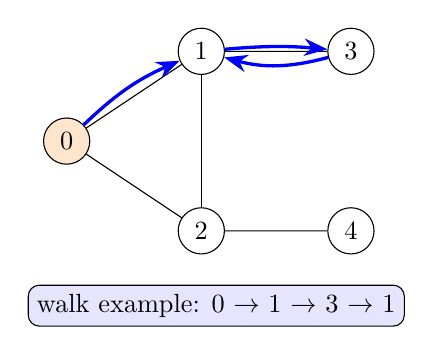
\begin{tikzpicture}[>=Stealth,scale=0.95,every node/.style={transform shape}]
\node[circle,draw,fill=orange!20] (n0) at (0,0) {0};
\node[circle,draw] (n1) at (1.8,1.2) {1};
\node[circle,draw] (n2) at (1.8,-1.2) {2};
\node[circle,draw] (n3) at (3.8,1.2) {3};
\node[circle,draw] (n4) at (3.8,-1.2) {4};
\draw (n0)--(n1)--(n3);
\draw (n0)--(n2)--(n4);
\draw (n1)--(n2);
\draw[->,very thick,blue] (n0) to[bend left=10] (n1);
\draw[->,very thick,blue] (n1) to[bend left=5] (n3);
\draw[->,very thick,blue] (n3) to[bend left=15] (n1);
\node[draw,rounded corners,fill=blue!10] at (2,-2.2) {walk example: 0 $\to$ 1 $\to$ 3 $\to$ 1};
\end{tikzpicture}
\end{center}
\end{frame}

\begin{frame}[fragile]{노트북의 random walk 구현}
\begin{lstlisting}
def random_walk(start, length):
    walk = [str(start)]
    for i in range(length):
        neighbors = [node for node in G.neighbors(start)]
        next_node = np.random.choice(neighbors, 1)[0]
        walk.append(str(next_node))
        start = next_node
    return walk
\end{lstlisting}
\begin{itemize}
  \item 반환값을 문자열로 두는 이유는 \texttt{Word2Vec} 입력 형식과 맞추기 위해서다.
  \item 한 번의 walk는 noisy하지만, 여러 번 반복하면 지역 구조가 안정적으로 드러난다.
\end{itemize}
\end{frame}

\begin{frame}{DeepWalk 알고리즘 요약}
\begin{enumerate}
  \item 모든 노드를 시작점 후보로 둔다.
  \item 각 노드에서 여러 개의 random walk를 생성한다.
  \item 생성된 walk 집합을 말뭉치(corpus)로 본다.
  \item Skip-gram / Word2Vec으로 노드 임베딩을 학습한다.
\end{enumerate}
\vspace{0.4em}
\[
\text{walks} = \{(v_1,v_2,\dots,v_L)\} \quad \Rightarrow \quad \text{Skip-gram training}
\]
\vspace{0.3em}
\begin{block}{해석}
같은 walk 문맥에 자주 등장하는 노드는 구조적으로 관련된 노드로 간주된다.
\end{block}
\end{frame}

\begin{frame}[fragile]{하이퍼파라미터가 의미하는 것}
\small
\begin{itemize}
  \item \textbf{walk length}: 한 시퀀스가 보는 구조 범위
  \item \textbf{walks per node}: 각 노드를 얼마나 자주 샘플링할지
  \item \textbf{window}: 문맥으로 인정할 주변 거리
  \item \textbf{embedding dimension}: 표현 용량
\end{itemize}
\vspace{0.4em}
\begin{lstlisting}
model = Word2Vec(walks,
                 hs=1,
                 sg=1,
                 vector_size=100,
                 window=10,
                 workers=1,
                 seed=1)
\end{lstlisting}
\end{frame}

\section{Karate Club 실습}

\begin{frame}[fragile]{노트북 2부: Karate Club 그래프}
\begin{itemize}
  \item \texttt{networkx.karate\_club\_graph()}는 고전적인 커뮤니티 분할 예제다.
  \item 라벨은 \texttt{Mr. Hi}와 \texttt{Officer} 두 클럽으로 구성된다.
  \item 구조만으로도 어느 정도 커뮤니티 분리가 가능하다는 점을 보여주기 좋다.
\end{itemize}
\vspace{0.3em}
\begin{lstlisting}
G = nx.karate_club_graph()
labels = []
for node in G.nodes:
    label = G.nodes[node]['club']
    labels.append(1 if label == 'Officer' else 0)
\end{lstlisting}
\end{frame}

\begin{frame}{실험 설정}
\begin{itemize}
  \item 노드마다 80개의 walk 생성
  \item 각 walk 길이: 10
  \item 임베딩 차원: 100
  \item 학습 후 세 가지를 확인
  \begin{itemize}
    \item 유사 노드 검색
    \item t-SNE 2차원 시각화
    \item RandomForest 기반 노드 분류
  \end{itemize}
\end{itemize}
\vspace{0.3em}
\begin{block}{의미}
DeepWalk는 비지도 표현학습이고, 분류기는 그 위에 얹는 다운스트림 태스크다.
\end{block}
\end{frame}

\begin{frame}[fragile]{유사도와 시각화 해석}
\begin{itemize}
  \item \texttt{most\_similar('0')}은 노드 0과 비슷한 문맥을 가진 노드를 찾는다.
  \item \texttt{wv.similarity('0', '4')}는 두 노드 임베딩의 코사인 유사도를 본다.
  \item t-SNE는 고차원 임베딩이 라벨별로 어느 정도 분리되는지 직관을 준다.
\end{itemize}
\vspace{0.4em}
\begin{lstlisting}
nodes_wv = np.array([model.wv.get_vector(str(i))
                     for i in range(len(model.wv))])
tsne = TSNE(n_components=2,
            learning_rate='auto',
            init='pca',
            random_state=0).fit_transform(nodes_wv)
\end{lstlisting}
\end{frame}

\begin{frame}[fragile]{다운스트림 분류 결과의 의미}
\begin{itemize}
  \item 학습 데이터는 12개 노드만 사용
  \item 테스트 데이터는 나머지 22개 노드
  \item 임베딩만으로도 커뮤니티 분류가 꽤 잘 되면,
  \item DeepWalk가 구조 정보를 유용한 feature로 압축했다는 뜻이다.
\end{itemize}
\vspace{0.4em}
\begin{lstlisting}
clf = RandomForestClassifier(random_state=0)
clf.fit(nodes_wv[train_mask], labels[train_mask])
y_pred = clf.predict(nodes_wv[test_mask])
acc = accuracy_score(y_pred, labels[test_mask])
\end{lstlisting}
\end{frame}

\section{정리}

\begin{frame}{Chapter 3 핵심 정리}
\begin{itemize}
  \item DeepWalk는 \textbf{NLP의 Word2Vec}을 \textbf{그래프 random walk}에 이식한 방법이다.
  \item 노드 임베딩은 비지도 방식으로 학습되고, 이후 분류/예측 태스크에 재사용된다.
  \item 좋은 임베딩은 같은 커뮤니티 혹은 비슷한 구조적 역할의 노드를 가깝게 둔다.
  \item 이는 이후 GCN, GraphSAGE 같은 GNN의 메시지 패싱 학습으로 자연스럽게 이어진다.
\end{itemize}
\end{frame}

\begin{frame}{다음 단계에서 생각할 질문}
\begin{itemize}
  \item 단순 random walk가 DFS/BFS 성향을 조절하지 못하는 한계는?
  \item 노드 feature가 있을 때는 DeepWalk만으로 충분한가?
  \item 비지도 임베딩과 end-to-end GNN의 장단점은 무엇인가?
\end{itemize}
\end{frame}

\end{document}
